% -*- root: ../../main.tex -*
%!TEX root = ../../main.tex
% vim:textwidth=80 fo=cqt conceallevel=0

% \afterpage{\clearpage}

\subsection{Introduction and guidelines for flow diagram traversal}

The  methodology adopted  by the  proposed layer  optimisation framework  can be
explained by  using the  flow diagram in  \cref{fig:fig_strategy_schematic}. The
power  handled by  the cell  during normal  operation (evaluated  by considering
various drivecycles)  is much  lower than  that experienced  during acceleration
(discharge)  and  fast-charging (charge)  scenarios.  \Cref{sec:resultslayeropt}
provides  a brief  summary of  the peak  and median  powers across  all standard
drivecycles. Therefore, from a design  perspective, it is sufficient to consider
the power  requirements for  these two  extreme cases.  Hence, the  schematic in
\cref{fig:fig_strategy_schematic} can  be studied  by broadly dividing  the flow
diagram into two parts ---
\begin{enumerate*}[label=\roman*)]
    \item an acceleration pathway (primarily consisting of blocks shaded in grey), and
    \item a fast-charging pathway (predominantly composed of blocks shaded in cyan).
\end{enumerate*}

\begin{figure}[p]
    \begin{minipage}[t]{\textwidth}
        \centering
        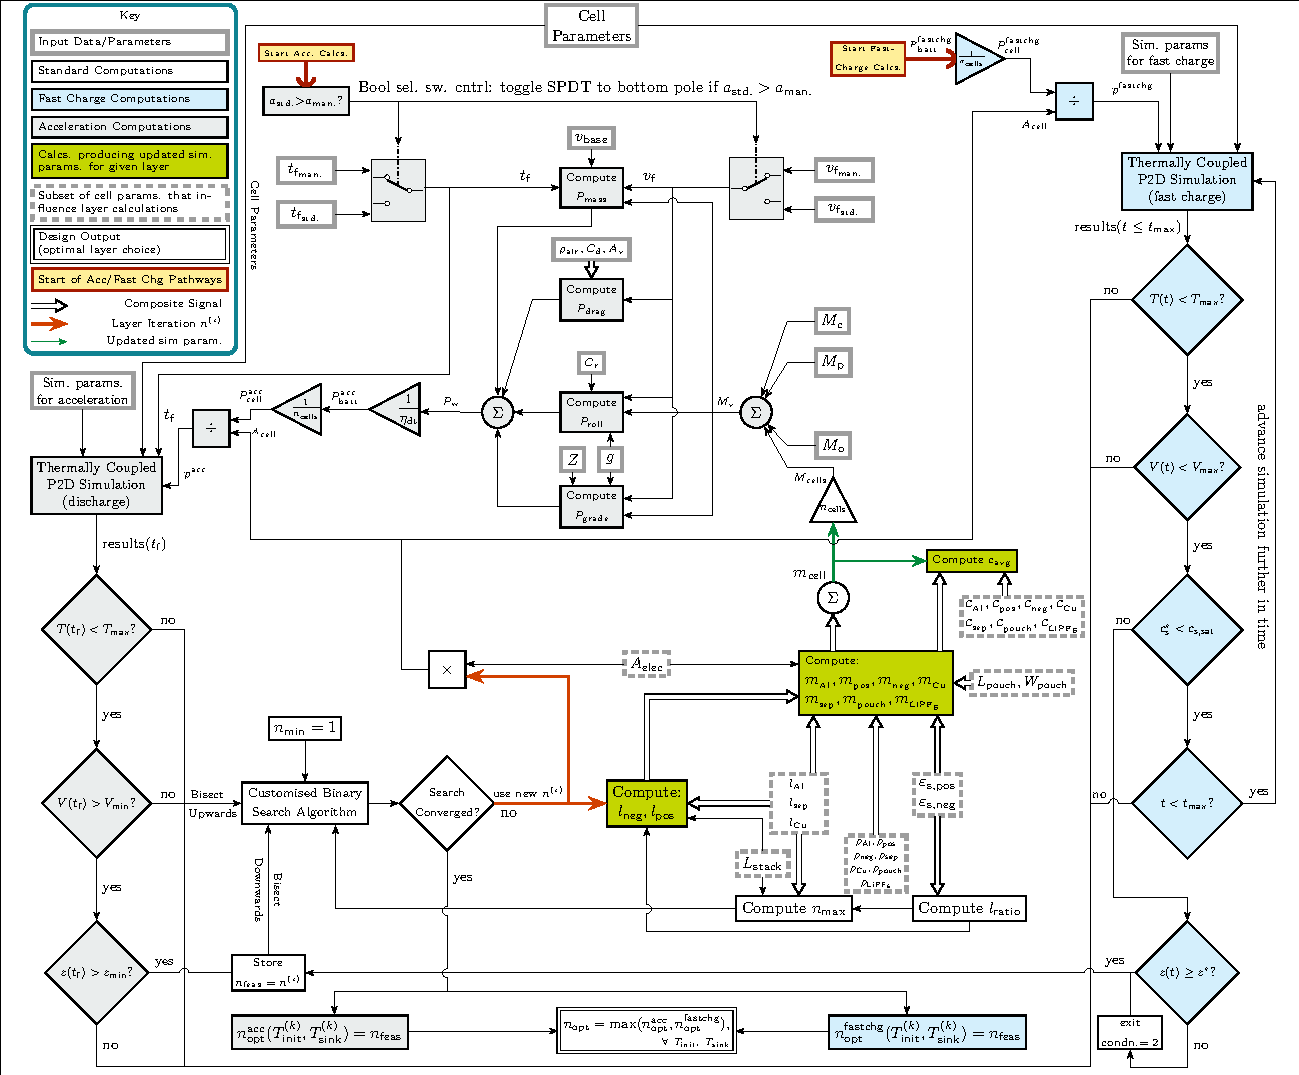
\includegraphics[angle=90, width=\textwidth]{fig_master_flow_diagram}
        \captionsetup{labelsep=note}
        \caption
        [%
        Flow diagram of layer optimisation methodology
        ]%
        {%
            Flow diagram depicting an overview of the proposed layer optimisation methodology
            for Li-ion pouch cells.
        }%
        \label{fig:fig_strategy_schematic}
        \mpfootnotes[1]
        % \vspace*{1.125cm}
        \vspace*{0.7225cm}
        \footnote{This figure was created by \mbox{Krishnakumar Gopalakrishnan} who
            asserts copyright, with intellectual contributions from and the right to
        use asserted by \mbox{Ian D.\ Campbell}.}
    \end{minipage}
\end{figure}

As indicated by  the legend in \cref{fig:fig_strategy_schematic},  blocks with a
light~grey border represent input  data/parameters for computations. Blocks with
a standard black  border represent computations common to  both acceleration and
fast charging pathways. The design output  is given by the double-bordered block
at  the  bottom  centre  of \cref{fig:fig_strategy_schematic}.  Other  types  of
blocks  and arrows  are  appropriately listed  in  the legend  key.  To aid  the
understanding of the  layer optimisation framework, the reader  is encouraged to
correlate  the narrative  in this  section  with the  blocks and  arrows in  the
schematic.  The  acceleration  and  fast  charging  pathways  are  not  amenable
for  standalone comprehension  and  are to  be parsed  in  conjunction with  the
flow  of  control through  the  infrastructure  blocks  as  if the  entire  flow
diagram  is a  single  cohesive unit.  These `control'  blocks,  common to  both
pathways  in \cref{fig:fig_strategy_schematic},  govern how  these two  pathways
are  to be  traversed  with the  presently trialled  layer  choice and  quantify
the  suitable  reformulations needed  whenever  a  new  layer  choice is  to  be
used.  The  computational aspects  covered  by  these  blocks are  described  in
\crefrange{sec:searchalgo}{sec:spheat}.

\subsection{Acceleration pathway}\label{sec:accpathway}

The computations for acceleration-based layer  optimisation begins at the anchor
block labelled `Start Acc.\ Calcs.'.

\subsubsection*{Determination of acceleration rate, final speed and acceleration time}

The  first  step is  to  determine  the rate  of  acceleration  to be  used  for
computing the power requirements for  accelerating an \gls{xeV} from standstill.
For  various  other  regulatory  reasons, vehicular  standards  for  electrified
transport are  codified by various  standardisation bodies (\eg~the SAE~J1772
standard~\cite{Sae2010}). The  standards published by these  regulatory agencies
typically specify  a minimum  required acceleration rate  for the  vehicle under
consideration  to be  certified as  an electric  vehicle. Additionally,  vehicle
manufacturers  often provide  their own  specifications, which  typically exceed
these minimum standards. However, for  certain classes of electric vehicles such
as golf carts,  the manufacturer-specified standards might fall below  that of a
roadworthy  electric vehicle.  This thesis  advocates a  conservative design  by
choosing the higher of the two values.

The  acceleration  rate  is  calculated   by  dividing  a  pre-determined  final
speed~$v_\text{f}$  by the  time~$t_\text{f}$ taken  to attain  that speed  from
standstill.  The  manufacturer-specified  acceleration  rate~$a_\text{man.}$  is
compared  against  the minimum  acceleration  rate  specified by  the  governing
vehicular   standards~$a_\text{std.}$.  The   two  \gls{spdt}   switches  assign
the  final  speed~$v_\text{f}$  and  acceleration  time~$t_\text{f}$  using  the
corresponding values from  the appropriate source depending on which  of the two
acceleration rates is higher.

\subsubsection*{Computation of acceleration power at the wheels}

The  next  step  is  to  calculate   the  acceleration  power  required  at  the
driving wheels~$P_\text{w}$.  Using the  governing equations from  basic vehicle
dynamics~\cite{Maksimovic2012}, the power at the wheels of an \gls{xeV} is given
by \cref{eq:wheelpower}.
\begin{subequations}\label{eq:wheelpower}
    \begin{align}
        \SwapAboveDisplaySkip
        P_\text{w}     & = P_\text{mass} + P_\text{drag} + P_\text{roll} + P_\text{grade} \tag{\ref*{eq:wheelpower}}                  \\
        P_\text{mass}  & = \frac{1}{2} \frac{M_\text{v}(n)}{t_\text{a}} \left(v_\text{b}^2 + v_\text{f}^2\right) \label{eq:masspower} \\
        P_\text{drag}  & = \frac{1}{2} \left(\rho_\text{air} C_\text{d} A_\text{v}v_\text{f}^3\right) \label{eq:dragpower}            \\
        P_\text{roll}  & = C_\text{r} M_\text{v}(n)\, g v_\text{f} \label{eq:rollpower}                                                 \\
        P_\text{grade} & = M_\text{v}(n)\, Z g v_\text{f} \label{eq:gradepower}
    \end{align}
\end{subequations}

The  individual  components  contributing   to  the  summation  for  wheel-power
computation   presented   in    \cref{eq:wheelpower}   is   briefly   explained.
$P_\text{mass}$~represents  the  power  required  to  accelerate  the  vehicle's
mass.   $P_\text{drag}$~and  $P_\text{roll}$~denote   the  powers   required  to
overcome   air  resistance   and  rolling   resistance  respectively.   Finally,
$P_\text{grade}$~represents  the power  required to  negotiate a  road gradient.
Except for $M_\text{v}(n)$  which is described next, all terms  in the \gls{rhs}
of \crefrange{eq:masspower}{eq:gradepower}  are constants. The  nomenclature for
each  of  these  terms   is  explained  in  tables~\ref{tbl:CommonVehicleParams}
and~\ref{tbl:UniqueVehicleParams}  along with  their  numerical  values used  in
simulation.

\subsubsection*{Computation of layer-dependent vehicle mass}\label{sec:layerdependentvehiclemass}

Changing  the layer  count used  within a  cell changes  its mass.  This in-turn
affects the mass of the pack, which further influences the overall vehicle mass.
Hence, for  precise computation  of~$P_\text{mass}$ in  \cref{eq:masspower}, the
vehicle's  mass is  computed  as a  function  of number  of  layers within  each
cell~$n$.

In  the  schematic  of \cref{fig:fig_strategy_schematic},  this  layer-dependent
calculation of  mass of all cells  in the pack~$M_\text{cells}$ is  shown by the
product of  the signal  labelled~$m_\text{cell}$ and  the triangular  gain block
representing the overall number of cells in the pack~$n_\text{cells}$.
\begin{equation}\label{eq:massofallcells}
    M_\text{cells} = n \times m_\text{cell}
\end{equation}

The  mass of  the vehicle  is  given by  the sum  of chassis  mass~$M_\text{c}$,
vehicle payload~$M_\text{p}$, pack overhead~$M_\text{o}$ and the layer-dependent
mass   of   all   cells   in   the  pack~$M_\text{cells}$   as   computed   in
\cref{eq:massofallcells}.   The   computation  of   mass   of   a  single   cell~$m_\text{cell}$ is detailed in \cref{sec:massofonecell}.

\subsubsection*{Computation of acceleration power density per layer}

Since the \gls{p2d} equations of the \gls{dfn} model are based upon a normalised
unit area and is  applicable only to each electrochemical layer,  the goal is to
compute the  power density experienced  by each layer. This  is arrived at  by a
sequence of simple scaling steps.

Firstly, the power demanded  at the pack terminals~$P^\text{acc}_\text{batt}$ is
computed  by  dividing  the  power  at  the wheels  by  the  efficiency  of  the
drivetrain.  As explained  in \cref{subsec:layeroptassumptions},  the drivetrain
consists of  a number  of components,  the efficiencies of  which depend  on the
operating point  (such as the  speed and torque  of the electric  motor, current
drawn  by the  power electronics  etc.). Following  the assumptions  detailed in
\cref{subsec:layeroptassumptions},  a single  lumped efficiency~$\eta_\text{dt}$
can be  used for the powertrain.  The power demand  on the pack is  then divided
by  the  number of  cells  in  the pack~$n_\text{cells}$  to  obtain the  power
demand  at the  input  of the  cell's terminals~$p^\text{acc}_\text{cell}$.  For
each  layer choice~$n$,  the overall  electrochemically active  surface area  is
computed  using by  using \cref{eq:overallarea},  wherein the  surface area  per
layer~$A_\text{elec}$ listed in \cref{tbl:lcoSimParamslayeropt} is held constant
throughout.  Finally, the  acceleration power  density per  layer~$p^\text{acc}$
is  computed  by  dividing  $p^\text{acc}_\text{cell}$ by  the  overall  surface
area~$A_\text{cell}$.

\subsubsection*{Thermally-coupled \glsfmtshort{p2d} simulation and exit
conditions}\label{sec:accexitconditions}

For  the  presently trialled  layer  choice~$n$,  a thermally-coupled  \gls{p2d}
simulation is performed for a duration  of $t_\text{f}$~seconds with the applied
power  density~$p^\text{acc}_\text{cell}$  corresponding  to  the present  layer
choice  as input  to  the  model. When  the  simulation  terminates, the  cell's
condition is compared against three criteria
\begin{enumerate}
    \item the maximum possible values of cell temperature~$T_\text{max}$,
    \item the minimum allowed terminal voltage~$V_\text{min}$, and
    \item the lowest allowed cell \gls{soc}~$z_\text{min}$.
\end{enumerate}
This helps  to determine  whether the  cell constructed  from the  present layer
choice is  able to  successfully satisfy the  acceleration power  demands. These
comparison operations are represented by  decision blocks placed in the leftmost
region of the schematic in \cref{fig:fig_strategy_schematic}.

If  any one  of the  three aforementioned  exit checks  fail, the  present layer
configuration is deemed  to be not feasible and the  entire workflow is repeated
by  trialling a  new  layer  choice. A  sophisticated  search  algorithm, to  be
described  in  \cref{sec:searchalgo}, is  employed  to  minimise the  number  of
iterations  needed  until  a successful  layer  choice~$n_\text{opt}^\text{acc}$
is  obtained.  The above  process  is  repeated  for different  combinations  of
initial and ambient temperatures~${(T_\text{init}, T_\text{sink})}$. The largest
successful  layer value  from  all  temperature combinations  is  deemed as  the
canonical  optimal design  choice  when considering  acceleration demands.  This
concludes the narrative describing the acceleration-specific pathway.


\subsection{Fast-charging pathway}\label{sec:fastchgpathway}

The  workflow describing  the optimal  layer calculation  for the  fast charging
scenario begins  with the  anchor block labelled  `Start Fast-Charge  Calcs.' in
\cref{fig:fig_strategy_schematic}. The charging algorithm used in this framework
is based  upon the model-based strategy  proposed by Choe~\etal~\cite{Choe2013},
wherein  the surface  concentration is  never allowed  to exceed  its saturation
value.  Adopting  this charging  scheme  leads  to  a  robust cell  design  that
is  resilient  to  lithium  plating.  A  major  departure  from  the  scheme  in
Choe~\etal~\cite{Choe2013}  is the  fact that  the constant  current phase  used
therein is replaced  by a constant power  phase. This is so  that the assumption
of  identical  conditions  across  all  cells   in  the  pack  holds  true  (see
\cref{subsec:layeroptassumptions} for  details). Furthermore, the  pulsing phase
used to  top-up the cell's  \gls{soc} in Choe~\etal~\cite{Choe2013}  is omitted.
This  is because,  the level~3  fast charging  specifications typically  require
charging to a  target \gls{soc} that is typically  well below \SI{100}{\percent}
(see \cref{tbl:lcoSimParamslayeropt}).

At     first,     the    charging     power     applied     at    the     pack's
terminals~$P_\text{batt}^\text{fastchg}$ is scaled down by the overall number of
cells in the pack.  This results in the charging power  experienced by each cell
in  the  pack~$P_\text{cell}^\text{fastchg}$.  Following the  strategy  used  in
\cref{sec:accpathway}, the power  at the cell's terminals is scaled  down by the
electrochemically active  overall surface area~$A_\text{cell}$. This  yields the
power density~$p^{\text{fastchg}}$ experienced by each  layer in the cell and is
now  amenable  to be  applied  to  the  normalised  \gls{p2d} equations  of  the
\gls{dfn} model (that has been suitably modified to handle power inputs).

\subsubsection*{Thermally-coupled fast-charging simulations and exit conditions}

After computing  the power  density per  layer, the  thermally-coupled \gls{p2d}
model  is  then  invoked.  While  the  simulation  runs,  the  cell's  state  is
continually evaluated against various termination criteria.
\begin{enumerate}
    \item the maximum possible values of cell temperature~$T_\text{max}$,
    \item the maximum allowed terminal voltage~$V_\text{max}$, and
    \item the surface concentration~$c_\text{s}^{\ast}$ not to exceed the saturation concentration~$\c_\text{s,sat}$
\end{enumerate}

If any  of these three criteria  are violated, the simulation  immediately stops
and the trialled layer  choice is deemed to not satisfy  the fast charging power
requirements. The  search algorithm then  updates the layer choice  suitably and
the entire workflow is repeated.

If the  simulation for  any layer choice  passes the  aforementioned termination
criteria,  the  \gls{soc}   achieved  by  the  cell  is   compared  against  the
fast-charging   target~$z^\ast$.  If~${z(t)   >  z^\ast}$,   then  the   present
layer  choice  represents   the  minimum  (and  therefore   optimum)  value  for
this  specific  fast  charging  application.  The  successful  layer  choice  is
labelled~$n_\text{opt}^\text{fastchg}$. If the surface concentration has not yet
reached the saturation limit, then the charge time is compared against the upper
bound for  fast charging specifications~$t_\text{max}$. If  this preset duration
has not been reached, then the simulation is allowed to advance further in time,
with the aforementioned  termination criteria being continuously  tested at each
subsequent time-step.

The above process is repeated for  different combinations of initial and ambient
temperatures~${(T_\text{init},  T_\text{sink})}$.  The  largest  successful
layer value from all temperature combinations is deemed as the canonical optimal
design choice when  considering the fast charging power  demands. This concludes
the  narrative describing  the  fast charging  pathway.

Finally, the  maximum of the  layer choices across all  temperature combinations
from the  acceleration and  fast charging  scenarios is  deemed as  the globally
optimal  number of  layers  to be  used  for this  model-led  cell design.  This
concludes the overall narrative describing the layer optimisation framework. The
results obtained by applying this methodology to a specific numerical example is
presented next in \cref{sec:resultslayeropt}.

% Do not forget to quote the value of cs_sat from layer opt paper table and show
% calculation inline. Might even go into the code

\subsection{Search algorithm}\label{sec:searchalgo}

A  customised binary  search algorithm  is designed  for the  layer optimisation
framework.  Binary  search  is  a  computationally  efficient  search  algorithm
requiring a worst-case  operational count of~$\mathcal{O}(\log k)$  where $k$~is
the  overall  number  of  layer  candidates  to  be  searched~\cite{Cormen2009}.
However, this  algorithm is  applicable only  when the array  to be  searched is
already  sorted in  either ascending  or  descending order.  By recognising  the
relationship between the  magnitude of power density applied  versus the factors
that deem a  layer suitable or unsuitable for the  application, a customised set
of `exit conditions'  that meet the aforementioned  sorted-array requirement can
be  enforced. This  specific  mapping is  a  unique  idea and  is  claimed as  a
contribution by this thesis author to the art.

This search  strategy is  equally applicable (with  small modifications  to exit
conditions as explained next) for both acceleration and fast charging pathways.

\subsubsection*{Binary search for acceleration pathway}

If all the termination criteria are  successfully met, the exit condition is set
to a  value of~1. If any  of these conditions  fail, then the exit  condition is
assigned a value of~0. Thus, the search vector in this bespoke strategy consists
of only two boolean possibilities. For ultra-low layer counts, the applied power
densities are extremely high. Therefore, one of the exit conditions is likely to
fail. For  very high layer  counts, the power  densities are very  low, implying
that acceleration runs shall always be successful. When considering layer counts
from  the lowest  to  the  highest, there  exists  a  critical transition  point
\viz~the  first layer  count  for which  the exit  vector  toggles from~0  to~1.
Through a systematic  bisection of the layer search space,  the search algorithm
speedily converges to the optimal layer value.

\subsubsection*{Binary search for fast-charging pathway}

If all  the fast-charging  termination criteria are  successfully met,  the exit
condition is  set to  a value  of~1. For  violating any  of the  following three
failure conditions (see \cref{sec:fastchgpathway}) \viz~exceeding
\begin{enumerate*}[label=\itshape\alph*\upshape)]
    \item upper cutoff temperature  and/or,
    \item upper cutoff voltage and/or
    \item the maximum allowed charging despite encountering surface saturation,
\end{enumerate*}
the exit condition is  assigned the value of~0. The search  array is bisected by
using  this failed  layer  choice as  the  new lower  bound.  If no  termination
criterion is  violated, then  the presently  trialled layer  choice is  deemed a
success and the exit condition is set to~1. The search space is narrowed down by
using the current layer choice as the new upper bound.

However,  there exists  an additional  third possibility  for the  fast charging
case.  If the  aforementioned termination  criteria  are not  violated, but  the
charging process fails to meet  the target \gls{soc} specification, this implies
that the number of layers used is too high (see \cref{fig:fig_CapacityQuadrants}
and \cref{sec:resultslayeropt} for  a brief explanation of this  case). The exit
condition corresponding to this failure mode is assigned a value of~2. Thus, the
search vector in this bespoke strategy  consists of three distinct numbered exit
conditions. Despite being a failure, from  the perspective of narrowing down the
search space,  exit condition~2 is treated  in the same way  as exit condition~1
\ie~the trialled layer choice is deemed to be too high.

Akin to the acceleration pathway, the  optimal layer choice for fast charging is
deemed to be at the critical transition point wherein the exit condition toggles
from 0~to~1 and  hence, minimal customisation is needed in  the computer code to
handle these two cases.  The handling of exit condition~2 is  shown in the lower
rightmost portion of \cref{fig:fig_strategy_schematic}. Despite being a failure,
from the search algorithms point of view  this is treated as a success, with the
only difference  being the  assignment of  the exit  condition value  purely for
logging and debugging purposes.

\subsubsection*{Alternative search algorithm --- linear search}

A  simpler alternative  to using  the binary  search algorithm  is the  standard
linear  search  algorithm. This  is  a  simple  search strategy  which  involves
sequentially iterating  from~$n_\text{min}$ to~$n_\text{max}$  until arriving at
the lowest  value~$n_\text{opt}^\text{acc}$  that satisfies all  the termination
criteria. However, a naive use of the linear search algorithm is computationally
expensive with a worst case operation count of~$\mathcal{O}(n)$. Therefore, this
thesis author  recommends the use  of the  bespoke binary search  algorithm. The
choice of minimum and maximum values for  the layer search space is discussed in
\cref{sec:layersearchbounds}.

\subsection{Upper and lower bounds on search space}\label{sec:layersearchbounds}


It is  helpful to determine  the highest possible number  of layers that  can be
physically  accommodated in  a stack  of height~$L_\text{stack}$.  For instance,
this value may be used as the  upper bound to the binary search algorithm (which
compulsorily requires  such an upper bound)  described in \cref{sec:searchalgo}.
This can be obtained by defining a  simple integer optimisation task as shown in
\cref{eq:maxlayersopt}. The objective function here  is to maximise the value of
the layer count~$n$  subject to the physical constraint that  the thicknesses of
both electrodes always remains positive.
\begin{equation}\label{eq:maxlayersopt}
    \begin{aligned}
        \underset{n \, \in \, \mathbb{N}}{\mathbf{max}} \quad & n                                                                                                                                              \\
        \text{s.t.} \quad                                     & l_\text{pos} = \left(\frac{L_\text{stack} - L_\text{Al}(n) - L_\text{Cu}(n) - n l_\text{sep}}{n(1 + l_\text{ratio})}\right) > 0 \\
                                                              & l_\text{neg} = \left(\frac{l_\text{ratio}(L_\text{stack} - L_\text{Al}(n) - L_\text{Cu}(n) - n
l_\text{sep})}{n(1 + l_\text{ratio})}\right) > 0
\end{aligned}
\end{equation}


\Cref{eq:analytical_nmax} represents the analytical  closed-form solution to the
integer optimisation problem of \cref{eq:maxlayersopt}.
\begin{equation}
    \label{eq:analytical_nmax}
    n_\text{max} = \max \left(\floor*{\frac{2\left(L_\text{stack} - l_\text{Cu}\right)}{l_\text{Al}+l_\text{Cu}+2 l_\text{sep}}}, \floor*{\frac{2L_\text{stack} - l_\text{Al} - l_\text{Cu}}{l_\text{Al} + l_\text{Cu} + 2l_\text{sep}}} \right)
\end{equation}

The  first   argument  to  the  $\max$~function  in  \cref{eq:analytical_nmax}
represents the maximum number of physically feasible odd layers while the second
argument  represents  the  maximum  such  value  when  considering  odd  layers.
Therefore, the greater of these two  values is chosen as the maximum permissible
layer choice~$n_\text{max}$ and is used as an input to the search algorithm.


In  the absence  of published  information on  how the  minimum layers  within a
pouch  cell is  currently set,  there is  presently no  unique way  to determine~$n_\text{min}$.  Therefore, for  this  layer optimisation  study,  the value  of
$n_\text{min}$ used  by the  search algorithm  is currently set  to one  --- the
minimum physically feasible number of layers. Design engineers from industry may
opt  to tweak  this to  a higher  value based  on insights  gained from  present
empirical designs.


% \subsubsection*{\hypertarget{href:layerdependentcellmass}{Computation of layer-dependent cell mass}}\label{sec:massofonecell}

\subsection{Electrode thickness ratio for capacity balancing}\label{sec:electroderatio}

A key idea of the layer optimisation  scheme is that, for computing the physical
lengths of  electrodes as a  function of number of  layers, the ratios  of their
thicknesses~$l_\text{ratio}$, is  held constant. This coefficient  is germane to
the concept  of capacity balancing of  electrodes with a view  to equalise their
loading. The  idea of matching  the capacity of  anode and cathode  materials is
widely accepted  as a standard principle  in cell design~\cite{Ramadesigan2012}.
The computation of this $l_\text{ratio}$ parameter is discussed here.

Equating  the active material volume of both electrodes,
\begin{equation}
    A_\text{elec,pos}l_\text{pos}  \varepsilon_\text{s,pos} = A_\text{elec,neg}l_\text{neg}  \varepsilon_\text{s,neg} \label{eq:electrodeCapacity}\\
\end{equation}

While  stacking the  layers  within a  pouch cell,  for  the negative  electrode
layers, there exists  an extra overhang of~${(<~\SI{2}{mm})}$ with  respect to the
positive  electrode layers.  \Cref{fig:anodeoverhangpouchcell}  shows a  CT~scan
depicting the two-dimensional longitudinal-sections with a close-up view of this
overhang region. This is a design feature  and helps to avoid plating of lithium
at the edges.

\begin{figure}[!htbp]
    \centering
    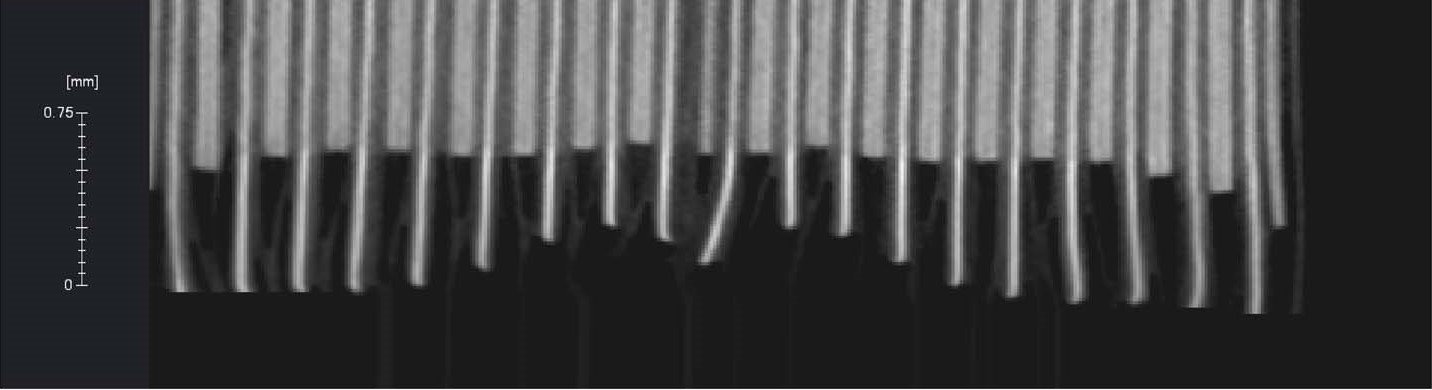
\includegraphics{overhang}
    \caption[Stacking of layers within a pouch cell showing overhang of negative
    electrode]
    {CT~scan showing the two-dimensional longitudinal-sections from the edge of
        the pouch cell with a close-up view of the graphite overhang region. For
        the negative electrode layers, there is an extra overhang of~${(<~\SI{2}{mm})}$ with respect to the positive electrode layers. This
        design feature helps to avoid plating of lithium at the edges. Image
    reproduced from Bond~\etal~\cite{Bond2017}.}
    \label{fig:anodeoverhangpouchcell}
\end{figure}

Neglecting   overhangs    of   the    negative   electrode    (typically   below
$\SI{2}{\milli\meter}$    to    avoid    plating    at    the    edges),    both
electrodes  have  the   same  cross-sectional  area~$A_\text{elec}$.  Therefore,
\cref{eq:electrodeCapacity} reduces to
\begin{align}
    \cancel{A_\text{elec}}l_\text{pos}  \varepsilon_\text{s,pos} & = \cancel{A_\text{elec}}l_\text{neg}  \varepsilon_\text{s,neg}  \\
    l_\text{pos}  \varepsilon_\text{s,pos}                       & = l_\text{neg}  \varepsilon_\text{s,neg}\label{eq:electrodeCapequalarea}
\end{align}

% For    the     reference    cell     under    consideration,     the    length
% and    breadth    of    the    cell's   pouch    is    obtained    from    the
% \gls{bev}    manufacturer~\cite{GMBoltBatteryDims}   and    are   listed    in
% \cref{tbl:lcoSimParamslayeropt}.

Owing to  the reasons outlined in  \cref{subsec:layeroptassumptions}, the volume
fractions  of  the  electrode  materials  are  assumed  to  be  constant,  which
implies  that  their   ratio  is  also  a  constant.   The  electrode  thickness
ratio~$l_\text{ratio}$ is therefore obtained as
\begin{alignat}{2}
    l_\text{ratio} & = \frac{l_\text{neg}}{l_\text{pos}}                                                                                  &  & \qquad\text{(by definition)}                                          \\
    {}             & = \frac{\varepsilon_\text{s,pos}}{\varepsilon_\text{s,neg}}                                                          &  & \qquad\text{(rearranging \cref{eq:electrodeCapequalarea})}           \\
    {}             & = \frac{1-\varepsilon_\text{pos} -
\varepsilon_\text{fi,pos}}{1-\varepsilon_\text{neg} - \varepsilon_\text{fi,neg}}
                   &  & \qquad\text{(by definition, see \cref{eq:volumefraccalc})}                                          \\
    {}             & = \frac{1- 0.385 - 0.025}{1 - 0.485 - 0.033}                                                                         &  & \qquad\text{(substituting values from \cref{tbl:lcoSimParamsSPMp2d})} \\
    l_\text{ratio} & = 1.22\label{eq:electrodeThicknessRatio}
\end{alignat}

\subsection{Computation of electrode thicknesses per layer}

In  this section,  a deterministic  way to  compute the  thickness of  electrode
materials is  present. In  the views  of this thesis  author, this  represents a
departure from  the norm wherein electrode  thicknesses are designed on  a trial
and  error basis~\cite{Ramadesigan2012}.  Following  the  assumptions listed  in
\cref{subsec:layeroptassumptions},  the exterior  dimensions  of  the pouch  are
held  constant. Furthermore,  as explained  in \cref{sec:surfareaperlayer},  the
thickness of  the electrochemical stack within  the pouch cell~$L_\text{stack}$,
is also considered to be constant.  Therefore, when the number of layers forming
the stack is varied,  this implies that the only quantities  that may be allowed
to change are the thicknesses of the two electrodes within each layer \ie~higher
the  layer  count, lower  the  electrode  thicknesses  and vice-versa.  In  this
section, this  relationship between the  number of layers~$n$ and  the electrode
thicknesses~$l_j\ (j  \in {\text{neg},\text{pos}})$ is quantified  with the help
of the key $l_\text{ratio}$ parameter obtained in \cref{sec:electroderatio}.

Figure~2 of Northrop~\etal~\cite{Northrop2011}  (suitably adapted and reproduced
in \cref{fig:topologies})  considers two possible configurations  of stacking up
layers within a pouch cell. In the first topology shown in \cref{fig:topology1},
the outermost current collectors are of copper. In the alternative configuration
shown in  \cref{fig:topology2}, a copper  current collector occupies one  end of
the  stack while  an aluminium  current collector  occupies its  other end.  The
formulae derived  here is equally applicable  to both these cases.  Although the
use of aluminium current collectors at both extrema of the stack is not studied,
the approach presented here may be easily extended to this case.

\begin{figure}[!htbp]
    \centering
    \begin{subfigure}[b]{0.725\textwidth}
        %
        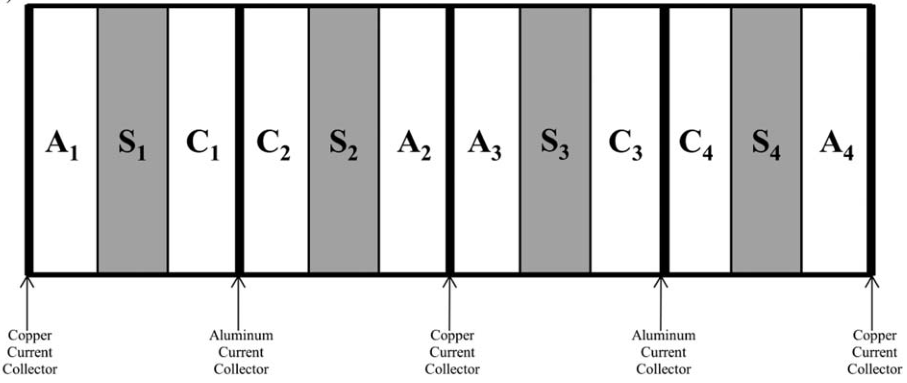
\includegraphics[width=\linewidth]{layer_stack2}
        %
        \caption{Topology 1}
        \label{fig:topology1}
    \end{subfigure}
    \hfill
    \begin{subfigure}[b]{0.225\textwidth}
        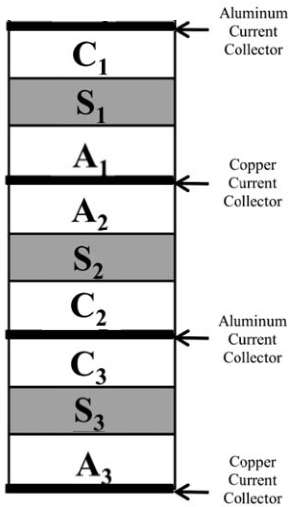
\includegraphics[width=\linewidth]{layer_stack}
        \caption{Topology 2}
        \label{fig:topology2}
    \end{subfigure}
    \caption[Two possile topologies for arranging the layers within a pouch
    cell]
    {Two possible topologies for arranging the layers within a pouch cell. The
        first possibility entails using an even number of layers as shown in the
        example illustration with four layers in the left sub-figure. Here, both
        extrema of the stack are occupied by copper current collectors. The
        second possible arrangement consists of using an odd number of layers
        and  is depicted in the  sample illustration with three layers in
        the right sub-figure. This represents a heterogeneous topology wherein
        the outermost current collectors of the stack consist of copper at one
        end and aluminium at its other end. Illustration adapted from
    Northrop~\etal~\cite{Northrop2011}.}
    \label{fig:topologies}
\end{figure}

The stack height  may be obtained by  the sum of thicknesses  of the constituent
regions.
\begin{align}
    L_\text{stack} &= \sum_jL_j(n) + L_\text{Al}(n) + L_\text{Cu}(n) \qquad\forall \ n \in \mathbb{N},\ j \in \{\text{pos, sep, neg}\} \label{eq:stackThickness}\\
    \shortintertext{where}
    L_j(n) &= n l_j\tag{\ref{eq:stackThickness}a}\\
    L_\text{Al}(n) &=
    \begin{cases}
        \left(\frac{n}{2}\right   )   l_\text{Al},& \text{if $n$ is even} \\
        \left(\frac{n+1}{2}\right )   l_\text{Al},& \text{if $n$ is odd}
    \end{cases}\tag{\ref{eq:stackThickness}b}\\
    L_\text{Cu}(n) &= \begin{cases}
        \left(\frac{n+2}{2}\right )  l_ \text{Cu},& \text{if $n$ is even}\\
        \left(\frac{n+1}{2}\right )  l_ \text{Cu},& \text{if $n$ is odd}\\
    \end{cases}\tag{\ref{eq:stackThickness}c}
\end{align}

The combined thickness of the  two electrode regions in each layer~$l_\text{ce}$
can be then obtained by rearranging \cref{eq:stackThickness}
\begin{equation}
    l_\text{ce} = \frac{L_\text{stack} - \ceil*{0.5(n+1)}l_\text{Cu} - \ceil*{0.5n}l_\text{Al}}{n} - l_\text{sep}\label{eq:combinedElectrodeThickness}\\
\end{equation}

The    individual     electrode    thicknesses    can    then     be    obtained
from   \cref{eq:combinedElectrodeThickness}   by    suitably   substituting   in
$l_\text{ratio}$ and performing simple algebraic manipulations.
\begin{align}
    l_\text{pos} &= \frac{l_\text{ce}}{l_\text{ratio}+1}\label{eq:lpos}\\
    l_\text{neg} &= l_\text{ce} - l_\text{pos}\label{eq:lneg}
\end{align}

The   values   of   the   two  electrode   thicknesses   thus   obtained   using
\Crefrange{eq:lpos}{eq:lneg}  are used  as computational  domain lengths  in the
\gls{p2d} simulations. Therefore,  these thicknesses have to  be recomputed each
time the trialled number of layers~$n$ is updated by the search algorithm.

\subsection{Computation of layer-dependent cell mass}\label{sec:massofonecell}

The mass of the cell varies as a  function of number of layers. This is because,
the thicknesses  of the  two electrodes  within each layer  changes each  time a
different layer choice is simulated. For a given layer choice~$n$, the cell mass
is computed as per \cref{eq:cellmass}.
\begin{subequations}\label{eq:cellmass}
\begin{align}
     m_\mathrm{cell} &= \sum\limits_{j}m_j + m_\mathrm{Al} + m_\mathrm{Cu} + m_\mathrm{LiPF_6} + m_\mathrm{pouch}, \; j \in  \{\text{pos, sep, neg}\}\tag{\ref*{eq:cellmass}}\\
     m_j &=   A_\mathrm{elec}  L_j \varepsilon_j\rho_j\label{eq:mj}\\
      m_\text{Al} &=   A_\mathrm{elec}  L_\text{Al} \rho_\text{Al}\label{eq:Almass}\\
      m_\text{Cu} &=   A_\mathrm{elec}  L_\text{Cu} \rho_\text{Cu}\label{eq:cumass}\\
      m_\mathrm{LiPF_6} &=   A_\mathrm{elec} \biggl(\sum\limits_{j} L_j (1-
      \varepsilon_{\text{fi}_j}-\varepsilon_j)\biggr)\rho_\mathrm{LiPF_6}\label{eq:lipf6mass} \\
      m_\mathrm{pouch} &= 2H_\mathrm{pouch} L_\mathrm{pouch} W_\mathrm{pouch}
      \rho_\mathrm{pouch}\label{eq:pouchmass}
 \end{align}
\end{subequations}


\Cref{eq:cellmass}   consists   of  both   constant   components   as  well   as
components   that  vary   with  the   number  of   layers.  For   instance,  the
mass  of  the  electrolyte~$m_\text{LiPF6}$  as   well  as  that  of  the  pouch
material~$m_\text{pouch}$ are constants and are computed only once.

\subsection{Computation of layer-dependent cell specific heat}\label{sec:spheat}

A lumped  thermal model of the  cell given by \cref{eq:thermalmodel}  is used to
model  the  thermal  dynamics  of  the  cell.  This  thermal  model  is  coupled
with  the  electrochemical  model  equations  of the  \gls{p2d}  model  for  the
simulations  used to  determine  the optimal  layer  configurations. The  cell's
temperature~$T_\text{cell}(t)$ is also obtained from this lumped thermal model.
\begin{align}
	m_\text{cell} c_\text{avg} \frac{dT_\text{cell}}{dt} &= -h A_\text{tabs} \left( T_\text{cell}(t) - T_\text{sink} \right) + Q_\text{pol} & \label{eq:thermalmodel}\\
	Q_\text{pol} &= A_\text{cell} \abs{i}\cdot \abs{U - V} & \tag{\ref{eq:thermalmodel}a}\\
	U &= U_\text{pos}(\theta_\text{pos})\big|_{\mathrlap{x = x_\text{pos/Alcc}}} \qquad - U_\text{neg}(\theta_\text{neg})\big|_{x = x_\text{neg/Cucc}} & \tag{\ref{eq:thermalmodel}b}\\
	V &= \phi_\text{s}\big|_{\mathrlap{x = x_\text{pos/Alcc}}} \qquad - \phi_\text{s}\big|_{x = x_\text{neg/Cucc}} & \tag{\ref{eq:thermalmodel}c}
\end{align}

The   average   specific   heat   of    the   cell~$c_\text{avg}$   used   in
\cref{eq:thermalmodel} is  a function of  the number of  layers and is  given by
\cref{eq:spheat}.
\begin{equation}\label{eq:spheat}
    c_\mathrm{avg} = \frac{1}{m_\text{cell}} \biggl[\sum_jc_jm_j + c_\text{Al}m_\text{Al} + c_\text{Cu}m_\text{Cu} + c_\mathrm{LiPF_6}m_\mathrm{LiPF_6} + c_\mathrm{pouch}m_\mathrm{pouch}\biggr],\quad j \in \{\text{pos, sep, neg}\}
\end{equation}

The first  three terms in  \cref{eq:spheat} are evaluated  as a function  of the
number of layers~$n$ by substituting the appropriate layer-dependent mass values
computed  in  \crefrange{eq:mj}{eq:cumass}.  The  latter  two  terms  \ie~the
specific heats of the electrolyte material and the pouch are held constant since
their corresponding mass values do not vary with the number of layers used.

